\documentclass[a4paper,10pt]{bxjsarticle}
\usepackage[dvipdfmx]{graphicx}
\usepackage{url}
\usepackage{amsmath}
\usepackage{amssymb}
\usepackage{amsfonts}
% \usepackage{here}

\title{プログラム演習 課題3}
\date{ }

\begin{document}

\maketitle

% \section*{section}

比誘電率$\epsilon_r$、厚さ$a$の誘電体スラブに沿ってz方向伝搬するTMモードの分散関係式を求める。

\begin{figure}[h]
    \centering
    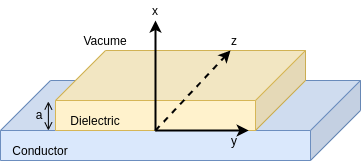
\includegraphics[width=0.5\textwidth]{fig.png}
    \caption{}
    \label{fig:1}
\end{figure}

$\rho = 0$とすると、Maxwell方程式は
\begin{eqnarray}
    \nabla \times \mathbb{E} &=& - \frac{\partial}{\partial t} \mathbb{B} \\
    \nabla \times \mathbb{B} &=&  \frac{\partial}{\partial t} \mu \epsilon \mathbb{E} \\
    \nabla \cdot \mathbb{E} &=& \frac{\rho}{\epsilon} = 0 \\
    \nabla \cdot \mathbb{B} &=& 0
\end{eqnarray}
となる。

(1)の両辺の回転をとる
\begin{align*}
    \nabla \times \left(\nabla \times \mathbb{E}\right)
        &= - \frac{\partial}{\partial t} \nabla \times \mathbb{B} \\
    \nabla \left(\nabla \cdot \mathbb{E}\right) - \nabla^2 \mathbb{E}
        &= - \frac{\partial}{\partial t} \frac{\partial}{\partial t} \mu \epsilon \mathbb{E} \\
    - \nabla^2 \mathbb{E}
        &= - \mu \epsilon \frac{\partial^2}{\partial t^2} \mathbb{E} \\
    \nabla^2 \mathbb{E} - \mu \epsilon \frac{\partial^2}{\partial t^2} \mathbb{E}
        &= 0 \tag{5} \\
\end{align*}

(2)の両辺で回転を取ると
\begin{align*}
    \nabla \times \left(\nabla \times \mathbb{B}\right)
        &= \mu \epsilon \frac{\partial}{\partial t} \nabla \times \mathbb{E} \\
    \nabla(\nabla \cdot \mathbb{B}) - \nabla^2 \mathbb{B}
        &= - \mu \epsilon \frac{\partial^2}{\partial t^2} \mathbb{B} \\
    \nabla^2 \mathbb{B} - \mu \epsilon \frac{\partial^2}{\partial t^2} \mathbb{B} 
        &= 0 \tag{6} \\
\end{align*}

$\frac{\partial}{\partial t} = j\omega$とすると式(5)(6)の Holmheltz方程式は
\begin{align*}
    \nabla^2 \mathbb{E} + \omega^2 \mu \epsilon \mathbb{E} &= 0 \\
    \nabla^2 \mathbb{B} + \omega^2 \mu \epsilon \mathbb{B} &= 0 \\
\end{align*}

TMモードより $E_z \neq 0, H_z = 0$
\begin{align*}
    \left( 
        \frac{\partial^2}{\partial x^2} 
        + \frac{\partial^2}{\partial y^2} 
        + \frac{\partial^2}{\partial z^2} 
    \right) H_y
    + \omega^2 \mu \epsilon H_y
    &= 0    
\end{align*}

z方向伝搬より $$H_y \propto e^{-\gamma z} = e^{-(\alpha + j \beta)z}$$ \\
無損失を仮定すると $\alpha = 0$なので $$H_y \propto e^{ -j \beta z}$$ \\
したがって、$ \frac{\partial}{\partial z} = -j \beta $ とすると
\begin{align*} 
    \left( 
        \frac{\partial^2}{\partial x^2} 
        + \frac{\partial^2}{\partial y^2} 
        - \beta^2 
    \right) H_y
    + \omega^2 \mu \epsilon H_y
    &= 0
\end{align*}

また、y方向に無限なスラブと仮定すると$\frac{\partial}{\partial y} = 0$となる。
\begin{align*} 
    \left( 
        \frac{\partial^2}{\partial x^2} 
        - \beta^2 
    \right) H_y
    + \omega^2 \mu \epsilon H_y
    &= 0
\end{align*}

$k^2 = -\beta^2 + \omega^2 \mu \epsilon$とおくと
\begin{align*} 
    \left( 
        \frac{\partial^2}{\partial x^2} 
        + k^2 
    \right) H_y
    &= 0
\end{align*}

したがって、誘電体中の$H_y$の一般解は
$$ H_y = A \sin k x + B \cos k x \qquad (A,B : const) $$

式(1)より
\begin{align*}
    \nabla \times \mathbb{B} 
    & = \begin{bmatrix}
        \frac{\partial}{\partial x}\\
        \frac{\partial}{\partial y}\\
        \frac{\partial}{\partial z}
    \end{bmatrix} \times
    \begin{bmatrix}
        0 \\
        \mu A \sin k x + \mu B \cos k x \\
        0 
    \end{bmatrix} \\
    & = \begin{bmatrix}
        - \frac{\partial}{\partial z}(\mu A \sin k x + \mu B \cos k x) \\
        0 \\
        \frac{\partial}{\partial x}(\mu A \sin k x + \mu B \cos k x)
    \end{bmatrix} \\
    & = \begin{bmatrix}
        j \mu \beta A \sin k x + j \mu \beta B \cos k x \\
        0 \\
        \mu k A \cos kx - \mu k B \sin kx 
    \end{bmatrix} \\
    &= \frac{\partial}{\partial t} \mu \epsilon \mathbb{E} \\
    &= - j \omega \mu \epsilon \mathbb{E} \\
    \\
    -j \omega \mu \epsilon E_x &= j \mu \beta A \sin k x + j \mu \beta B \cos k x \\
    E_x &= -\frac{\beta}{\omega \epsilon} A \sin k x -\frac{\beta}{\omega \epsilon} B \cos k x \\
    \\
    E_y &= 0 \\
    \\
    -j \omega \mu \epsilon E_z &= - \mu k A \cos kx + \mu k B \sin kx  \\
    E_z &= - \frac{k}{j \omega \epsilon} A \cos kx + \frac{k}{j \omega \epsilon} B \sin kx \\
\end{align*}

誘電体中での一般解をまとめると
\begin{align*}
    \begin{cases}
        E_x &= -\frac{\beta}{\omega \epsilon} A \sin k x -\frac{\beta}{\omega \epsilon} B \cos k x \\
        E_y &= 0 \\
        E_z &= -\frac{k}{j \omega \epsilon} A \cos kx + \frac{k}{j \omega \epsilon} B \sin kx
    \end{cases} \qquad
    \begin{cases}
        H_x &= 0 \\
        H_y &= A \sin k x + B \cos k x \\
        H_z &= 0
    \end{cases}
\end{align*}

導体中は$\mathbb{E} = \mathbb{B} = 0$となるので、
境界条件より電場$\mathbb{E}$の接線成分は$0$になるため
\begin{align*}
    E_z|_{x=0} &= -\frac{k}{j \omega \epsilon} A = 0 \\
    \therefore A &= 0
\end{align*}
よって
\begin{align*}
    \begin{cases}
        E_x &= -\frac{\beta}{\omega \epsilon} B \cos k x \\
        E_y &= 0 \\
        E_z &= \frac{k}{j \omega \epsilon} B \sin kx
    \end{cases} \qquad
    \begin{cases}
        H_x &= 0 \\
        H_y &= B \cos k x \\
        H_z &= 0
    \end{cases}
\end{align*}

また、真空中の場合、(5)(6)のHolmheltz方程式は
\begin{align*}
    \nabla^2 \mathbb{E} + \omega^2 \mu_0 \epsilon_0 \mathbb{E} &= 0 \\
    \nabla^2 \mathbb{B} + \omega^2 \mu_0 \epsilon_0 \mathbb{B} &= 0 \\
\end{align*}

誘電体スラブ中と同様に$H_y$について解くと
\begin{align*}
    \left( \frac{\partial^2}{\partial x^2} - \beta^2 \right) H_y + \omega^2 \mu_0 \epsilon_0 H_y &= 0
\end{align*}

ここで$k_0^2 = \beta^2 - \omega^2 \mu_0 \epsilon_0$とすると
\begin{align*}
    \left( \frac{\partial^2}{\partial x^2} - k_0^2 \right) H_y &= 0 \\
    H_y &= C e^{\pm k_0 (x - a)} \qquad ( C : const)
\end{align*}

$x \rightarrow \infty$の境界条件を考えると
$$ \lim_{x \to \infty} H_y = 0 $$ より
$$ H_y = C e^{- k_0 (x - a)} $$

式(1)より
\begin{align*}
    \nabla \times \mathbb{B} 
    & = \begin{bmatrix}
        \frac{\partial}{\partial x}\\
        \frac{\partial}{\partial y}\\
        \frac{\partial}{\partial z}
    \end{bmatrix} \times
    \begin{bmatrix}
        0 \\
        \mu_0 C e^{- k_0 (x - a)} \\
        0 
    \end{bmatrix} \\
    & = \begin{bmatrix}
        -\frac{\partial}{\partial z} \mu_0 C e^{- k_0 (x - a)} \\
        0 \\
        \frac{\partial}{\partial x} \mu_0 C e^{- k_0 (x - a)}
    \end{bmatrix} \\
    & = \begin{bmatrix}
        j\beta \mu_0 C e^{- k_0 (x - a)} \\
        0 \\
        - k_0 \mu_0 C e^{- k_0 (x - a)}
    \end{bmatrix} \\
    &= -j \omega \mu_0 \epsilon_0 \mathbb{E} \\
    \\
    j\omega \mu_0 \epsilon_0 E_x &= j\beta \mu_0 C e^{- k_0 (x - a)} \\
    E_x &= \frac{\beta}{\omega \epsilon_0} C e^{- k_0 (x - a)} \\
    \\
    j\omega \mu_0 \epsilon_0 E_z &= k_0 \mu_0 C e^{- k_0 (x - a)} \\
    E_z &= \frac{k_0}{j\omega \epsilon_0} C e^{- k_0 (x - a)}
\end{align*}

真空中の一般解をまとめると
\begin{align*}
    \begin{cases}
        E_x &= \frac{\beta}{\omega \epsilon_0} C e^{- k_0 (x - a)} \\
        E_y &= 0 \\
        E_z &= \frac{k_0}{j\omega \epsilon_0} C e^{- k_0 (x - a)}
    \end{cases} \qquad
    \begin{cases}
        H_x &= 0 \\
        H_y &= C e^{- k_0 (x - a)} \\
        H_z &= 0
    \end{cases}
\end{align*}

$x=a$での境界条件より、$\mathbb{E}$と$\mathbb{H}$の接線成分は連続なので
\begin{align*}
    \begin{cases}
        E_z |_{x=a} &= -\frac{k}{j\omega \epsilon} B \sin ka = \frac{k_0}{j\omega \epsilon_0}C \\
        H_y |_{x=a} &= B \cos ka = C 
    \end{cases} \\
\end{align*}
\begin{align*}
    -\frac{\epsilon_0}{\epsilon} \frac{k}{k_0} B \sin ka &= B \cos ka \\
    \tan ka &= - \frac{\epsilon}{\epsilon_0} \frac{k_0}{k}\\
            &= - \epsilon_r \frac{k_0}{k} \\
    \tan (\sqrt{-\beta^2+\omega^2 \mu \epsilon}\ a) &= - \epsilon_r \sqrt{\frac{-\beta^2+\omega^2 \mu \epsilon}{\beta^2-\omega^2 \mu_0 \epsilon_0}}
\end{align*}

$x = \beta a,\ y = \omega a /c$と規格化すると、
光速$\frac{1}{c} = \sqrt{\mu_0 \epsilon_0} $より
\begin{align*}
    \tan (\sqrt{-\beta^2+\omega^2 \mu \epsilon}\ a) &= - \epsilon_r \sqrt{\frac{-\beta^2+\omega^2 \mu \epsilon}{\beta^2-\omega^2 \mu_0 \epsilon_0}} \\
    \tan (\sqrt{-\beta^2 a^2+\omega^2 a^2 \mu \epsilon} ) &= - \epsilon_r \sqrt{\frac{-\beta^2 a^2 +\omega^2 a^2 \mu \epsilon}{\beta^2 a^2 - \omega^2 a^2 \mu_0 \epsilon_0}} \\
    \tan (\sqrt{-x^2 + \epsilon_r y^2 } ) &= - \epsilon_r \sqrt{\frac{-x^2 + \epsilon_r y^2}{ x^2 - y^2}} \\
\end{align*} 

比較のため、真空のみの場合を考える

$a \rightarrow 0,\ \epsilon_r = 1$とすると分散関係式は
\begin{align*}
    \tan 0 &= - \sqrt{\frac{-x^2 + y^2}{ x^2 - y^2}} \\
    -x^2 + y^2 &= 0 \\
    y^2 &= x^2 \\ 
    y = x
\end{align*}

また、誘電体のみの場合を考えると、分散関係式は
\begin{align*}
    \tan 0 &= - \epsilon_r \sqrt{\frac{-x^2 + \epsilon_r y^2}{ x^2 - y^2}} \\
    -x^2 + \epsilon_r y^2 &= 0 \\
    y^2 &= x^2 / \epsilon_r \\ 
    y = x / \sqrt{\epsilon_r}
\end{align*}

\newpage

電磁界分布を求める。
単位面積あたりの伝送電力で規格化する。

誘電体中の複素Poyntingベクトルは
\begin{align*}
    \mathbb{P} &= \mathbb{E} \times \mathbb{B}^* \\
    &= \begin{bmatrix}
        - \frac{\beta}{\omega \epsilon} B \cos kx \\
        0 \\
        -\frac{k}{j\omega \epsilon} B \sin kx
    \end{bmatrix} \times
    \begin{bmatrix}
        0 \\
        B \cos kx \\
        0
    \end{bmatrix} \\
    &= \begin{bmatrix}
        \frac{k}{j\omega \epsilon} B \sin kx \cdot B \cos kx \\
        0 \\
        - \frac{\beta}{\omega \epsilon} B \cos kx \cdot B \cos kx 
    \end{bmatrix} \\
\end{align*}

$xy$平面での単位面積当たりの有効伝送電力$P_e$は
\begin{align*}
    P_e &= | Re \left[ \mathbb{P} \right] | \\
    &= \sqrt{ \left(-\frac{\beta}{\omega \epsilon} B^2 \cos^2 kx \right)^2} \\
    &= \frac{\beta}{\omega \epsilon} B^2 \cos^2 kx \\
\end{align*}

真空中の複素Poyntingベクトルは
\begin{align*}
    \mathbb{P} &= \mathbb{E} \times \mathbb{H}^* \\ 
    &= \begin{bmatrix}
        -\frac{\beta}{\omega \epsilon_0} C e^{-k_0(x-a)} \\
        0 \\
        \frac{k_0}{j\omega \epsilon_0} C e^{-k_0(x-a)}
    \end{bmatrix} \times
    \begin{bmatrix}
        0 \\
        C e^{-k_0(x-a)} \\
        0
    \end{bmatrix} \\
    &= \begin{bmatrix}
        -\frac{k_0}{j\omega \epsilon_0} C e^{-k_0(x-a)} \cdot C e^{-k_0(x-a)} \\
        0 \\
        -\frac{\beta}{\omega \epsilon_0} C e^{-k_0(x-a)} \cdot C e^{-k_0(x-a)}
    \end{bmatrix} \\
    &= \begin{bmatrix}
        -\frac{k_0}{j\omega \epsilon_0} C^2 e^{-2k_0(x-a)} \\
        0 \\
        -\frac{\beta}{\omega \epsilon_0} C^2 e^{-2k_0(x-a)}
    \end{bmatrix} \\
\end{align*}

$xy$平面での単位面積当たりの有効伝送電力$P_e$は
\begin{align*}
    P_e &= | Re \left[ \mathbb{P} \right] | \\
    &= \sqrt{ \left( -\frac{\beta}{\omega \epsilon_0} C^2 e^{-2k_0(x-a)} \right)^2} \\
    &= \frac{\beta}{\omega \epsilon_0} C^2 e^{-2k_0(x-a)} \\
\end{align*}

単位幅あたりの有効伝送電力が$1$になるように規格化する
\begin{align*}
    \int_0^\infty P_e \,dx 
    &= \int_0^a P_e \,dx + \int_a^\infty P_e \,dx\\
    &= \int_0^a \frac{\beta}{\omega \epsilon} B^2 \cos^2 kx  \,dx 
     + \int_a^\infty \frac{\beta}{\omega \epsilon_0} C^2 e^{-2k_0(x-a)} \,dx\\
    &= \frac{\beta}{\omega \epsilon} B^2 \int_0^a \frac{1+\cos 2kx}{2}  \,dx 
     + \frac{\beta}{\omega \epsilon_0} C^2 \int_a^\infty  e^{-2k_0(x-a)} \,dx\\
    &= \frac{\beta}{2\omega \epsilon} B^2 \left[ x + \frac{1}{2k} \sin 2kx \right]_0^a 
     + \frac{\beta}{\omega \epsilon_0} C^2 \left[ -\frac{1}{2k_0} e^{-2k_0(x-a)} \right]_a^\infty \\
    &= \frac{\beta}{2\omega \epsilon} B^2 \left( a + \frac{1}{2k} \sin 2ka \right)
     + \frac{\beta}{\omega \epsilon_0} C^2 \cdot \frac{1}{2k_0} \\
    &= \frac{\beta}{2\omega \epsilon} B^2 \left( a + \frac{1}{2k} \sin 2ka \right) + \frac{\beta}{2k_0 \omega \epsilon_0} C^2 \\
    &= 1
\end{align*}

誘電体-真空の境界条件より$C = B \cos ka$
\begin{align*}
    \frac{\beta}{2\omega \epsilon} B^2 \left( a + \frac{1}{2k} \sin 2ka \right) 
        + \frac{\beta}{2k_0 \omega \epsilon_0} C^2 &= 1 \\
    \frac{\beta}{2\omega \epsilon} B^2 \left( a + \frac{1}{2k} \sin 2ka \right) 
        + \frac{\beta}{2k_0 \omega \epsilon_0} B^2 \cos^2 ka &= 1 \\
    B^2 \left[
        \frac{\beta}{2\omega \epsilon} \left( a + \frac{1}{2k} \sin 2ka \right) 
            + \frac{\beta}{2k_0 \omega \epsilon_0} \cos^2 ka
    \right] &= 1 \\
    B^2 \cdot \frac{\beta}{2\omega \epsilon}\left(
         a + \frac{1}{2k} \sin 2ka + \frac{\epsilon_r}{k_0} \cos^2 ka
    \right) &= 1 \\
    B^2 &= \frac{2\omega \epsilon}{\beta}\left(
        a + \frac{1}{2k} \sin 2ka + \frac{\epsilon_r}{k_0} \cos^2 ka
   \right)^{-1}\\
   B &= \sqrt{\frac{2\omega \epsilon}{\beta}\left(
    a + \frac{1}{2k} \sin 2ka + \frac{\epsilon_r}{k_0} \cos^2 ka
\right)^{-1}}\\
\end{align*}


%===========================================================================
% \cite{aaa}
% \begin{thebibliography}
%     \bibitem{aaa} aaa \url{url}
% \end{thebibliography}

% \begin{table}[htb]  
%     \centering
%     \caption{table}
%     \begin{tabular}{|c|c|c|} \hline
%         a & b & c \\\hline
%         1 & 2 & 3 \\\hline
%     \end{tabular}
% \end{table}

%   \begin{figure}[h]
%       \centering
%       \includegraphics[width=0.7\textwidth]{  }
%       \caption{}
%       \label{fig:}
%   \end{figure}
  
\end{document}